\chapter{The Design and Development of the Immotion Exergame}\label{chapter:implementation}

This chapter outlines the design and development of the Immotion exergame for warm up routine guidance and motivation. We begin with the description of the design methodology used for the development. For the purpose of this thesis, an iterative and prototype driven, user centered design has been adopted. Next, we cover the main development iterations
that have been undertaken during the exergame development process. 

\subsection{Overview of User Centered Design}

\subsection{Overview of the Development Phases}
The development of the Immotion exergame consisted of three primary phases which are according to the well accepted game design phases outlined by Furher and are depicted in Figure \ref{fig:iterations}: 
\begin{itemize}
\item Requirements gathering 
\item First prototype development with user evaluation
\item Final exergame development with further user evaluation
\end{itemize}
In the following sections, each iteration presented in Development section of Figure \ref{fig:iterations} will be further detailed. 
\begin{figure}[h]
    \centering
    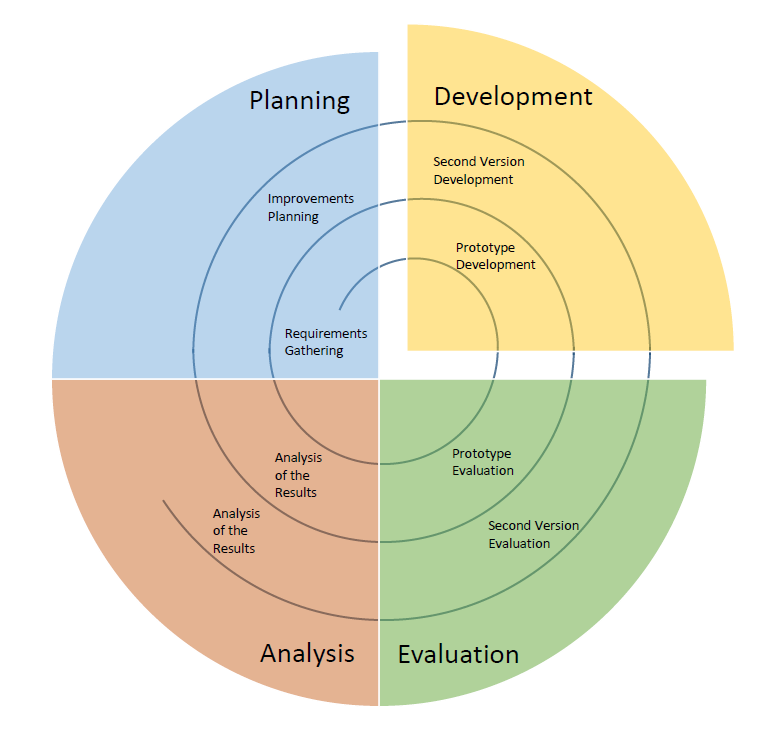
\includegraphics[width=\textwidth]{iterations}
    \caption{Overview of the development iterations}
    \label{fig:iterations}
\end{figure}
\section{Requirements Gathering}
This iteration was an exploratory step that justified the development and identified the currently available solution in the domain of exergames for warm up before sports activities. This was achieved through initial literature review which identified the most important areas to be addressed when developing gamified solution in the given context. TODO. Discussions with TAs?
\section{Prototype Development}
This section outlines the development of the prototype version of the exergame for warm up before sports activities. Our primary goal with the prototype was to develop a working version of the game that can process movements in real time in order to guide users through the warm up routine and, presumably make the routine more enjoyable and engaging.

\subsection{Game Description}
\subsection{Game Scenes}
\section{Final Exergame Solution}